\documentclass[border=10pt]{standalone}

\usepackage{tikz}
\usepackage{tikzsymbols}
\usetikzlibrary{calc,patterns,shapes.geometric}

\def\centerarc[#1](#2)(#3:#4:#5){\draw[#1] ($(#2)+({#5*cos(#3)},{#5*sin(#3)})$) arc (#3:#4:#5);}

\begin{document}
	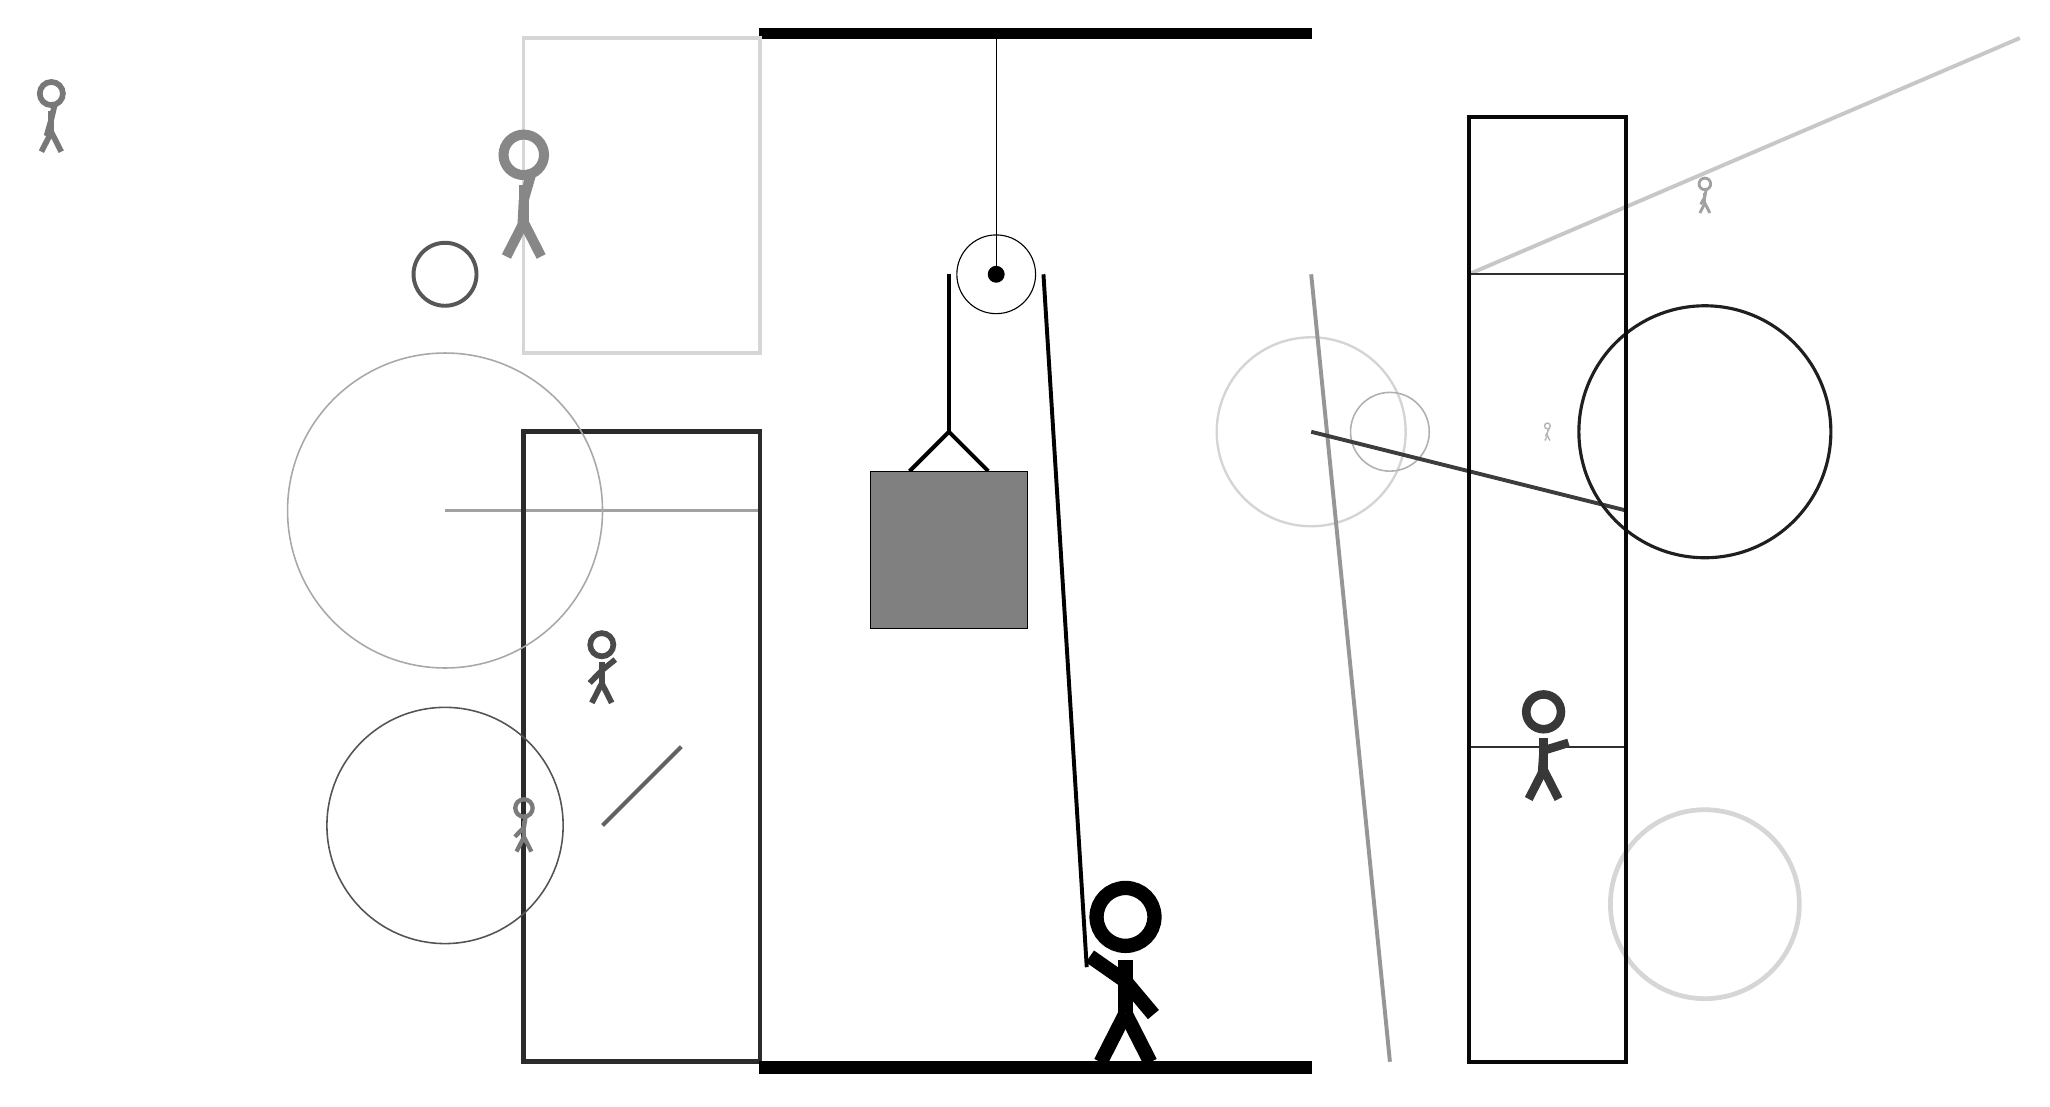
\begin{tikzpicture}
		%%%%% START %%%%%
		
		\draw[fill=black] (-2, 10) rectangle (5, 10.125);
		
		\draw (1, 7) circle (0.5);
		\draw[fill=black] (1, 7) circle (0.1);
		\draw (1, 10) -- (1, 7);
		
		\draw[line width=0.5mm] (-0.1, 4.5) -- (0.4, 5.0) -- (0.9, 4.5);
		\draw[fill=black!50] (-0.6, 4.5) rectangle (1.4, 2.5);
		
		\draw [line width=0.5mm, color=black!66](-6, 7) circle (0.4);
		
		\node[line width=0.5mm, color=black!71] at (-4, 2) {\Strichmaxerl[4][46][39]};
		\draw[line width=0.5mm, color=black!37](-6, 4) -- (-2, 4);
		\draw[line width=0.5mm, color=black!22](7, 7) -- (14, 10);
		\draw [line width=0.3mm, color=black!17](5, 5) circle (1.2);
		
		\node[line width=0.7mm, color=black!53] at (-11, 9) {\Strichmaxerl[4][74][77]};
		\draw[line width=0.5mm, color=black!41](5, 7) -- (6, -3);
		
		\draw[line width=0.5mm, color=black!61](-4, 0) -- (-3, 1);
		\draw[line width=0.6mm, color=black!83] (-2, -3) rectangle (-5, 5);
		\draw [line width=0.2mm, color=black!31](6, 5) circle (0.5);
		
		\draw[line width=0.5mm, color=black!76](5, 5) -- (9, 4);
		\draw[line width=0.4mm, color=black!16] (-2, 6) rectangle (-5, 10);
		\draw [line width=0.2mm, color=black!34](-6, 4) circle (2.0);
		
		\draw [line width=0.2mm, color=black!67](-6, 0) circle (1.5);
		\node[line width=0.6mm, color=black!37] at (10, 8) {\Strichmaxerl[2][61][80]};
		\draw [line width=0.4mm, color=black!88](10, 5) circle (1.6);
		\node[line width=0.2mm, color=black!52] at (-5, 0) {\Strichmaxerl[3][46][81]};
		\draw[line width=0.3mm, color=black!81] (7, 7) rectangle (9, 1);
		\node[line width=0.4mm, color=black!29] at (8, 5) {\Strichmaxerl[1][62][67]};
		
		\node[line width=0.7mm, color=black!47] at (-5, 8) {\Strichmaxerl[7][87][74]};
		\node[line width=0.4mm, color=black!78] at (8, 1) {\Strichmaxerl[6][86][17]};
		
		\draw [line width=0.6mm, color=black!16](10, -1) circle (1.2);
		\draw[line width=0.5mm, color=black!97] (7, -3) rectangle (9, 9);
		
		\draw[line width=0.5mm] (0.4, 7) -- (0.4, 5.0);
		\centerarc[line width=0.5mm](1, 7)(0:180:0.6);
		\draw[line width=0.5mm](1.6, 7) -- (2.15, -1.8);
		
		\node at (2.6, -1.9) {\Strichmaxerl[10][-35][-50]};
		
		\draw[fill=black] (-2, -3) rectangle (5, -3.15);
		
		%%%%% END %%%%%
	\end{tikzpicture}
\end{document}